\documentclass[11pt,a4paper]{article}
\usepackage[a4paper,hmargin=1in,vmargin=1in]{geometry}
\usepackage{pgfplots}
\pgfplotsset{compat=1.17}

\usepackage[british]{babel}
\usepackage[utf8]{inputenc}
\usepackage[T1]{fontenc}

\usepackage[nodayofweek]{datetime}
\newdate{date}{19}{3}{2024}

\usepackage{stddoc}
\usepackage{lipsum}


\begin{document}

    \pagenumbering{arabic}

    % Header
    \begin{center}
        {\LARGE\textbf{Application of FinFET technology in RF systems}}\\[3mm]
        \begin{minipage}{0.4\textwidth}
            \begin{flushleft}
                \textsc{\displaydate{date}}
            \end{flushleft}
        \end{minipage}
        ~
        \begin{minipage}{0.4\textwidth}
            \begin{flushright}
                \textsc{Martin Šimák}
            \end{flushright}
        \end{minipage} 
        \noindent\rule{14.5cm}{0.4pt}
    \end{center}

    \section{Introduction}

        Recent technological trends indicate a shift towards higher frequencies in the field of electronic engineering, which imposes new requirements on the radio-frequency (RF) capabilities of developed components. With the integration of additional components into LTE phones and the emergence of novel sub-6-GHz 5G bands, the need for area scaling becomes crucial to accommodate a variety of chipsets within compact cellphone designs, all while ensuring optimal power efficiency.
    
        FinFET-based logic process technologies have risen as a favoured option for production, boasting significant advantages including exceptional scalability, minimal power consumption, and outstanding performance, especially evident at 14-nm and 16-nm nodes.


    \section{Performance}

        Working with the data provided in~\cite{singh:14nm-finfet-analog-and-rf-applications}, we can make a direct performance comparison in the following three crucial RF figures of merit:
        \begin{itemize}
            \item $f_{\mathrm{t}}$ as the cutoff frequency, i.e., the frequency at which the magnitude of the current gain has dropped to unity (i.e., $\qty{0}{\dB}$);
            \item $f_{\mathrm{max}}$ as the maximum frequency of oscillation, i.e., the frequency at which the unilateral power gain equals unity (i.e., $\qty{0}{\dB}$);
            \item $G_{\mathrm{m}}/G_{\mathrm{ds}}$ as the self-gain, where $G_{\mathrm{m}}$ is the transconductance and $G_{\mathrm{ds}}$ is the output conductance.
        \end{itemize}

        For most RF applications, power gain and $f_{\mathrm{max}}$ are more important than current gain and $f_{\mathrm{t}}$. However, that is not always the case, and we should inspect both parameters, as displayed in Figure~\ref{fig:performance-frequencies}. These plots are taken from~\cite{singh:14nm-finfet-analog-and-rf-applications}, and they display the frequency performance using a minimum channel length (14 nm), 12-fin N-type and P-type FinFET devices. The measurements were taken using the open, short and through de-embedding technique for the elimination of the pad and the interconnect effects.
        \begin{figure}[!ht]
            \centering
            \begin{subfigure}{.45\textwidth}
                \centering
                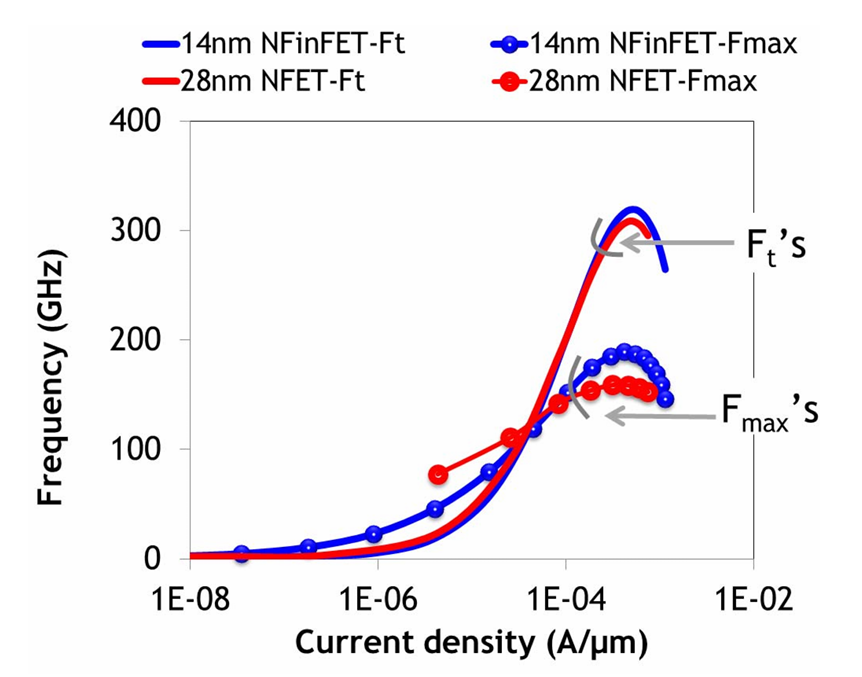
\includegraphics[width=\textwidth]{src/frequencies-ntype.png}
            \end{subfigure}
            ~
            \begin{subfigure}{.45\textwidth}
                \centering
                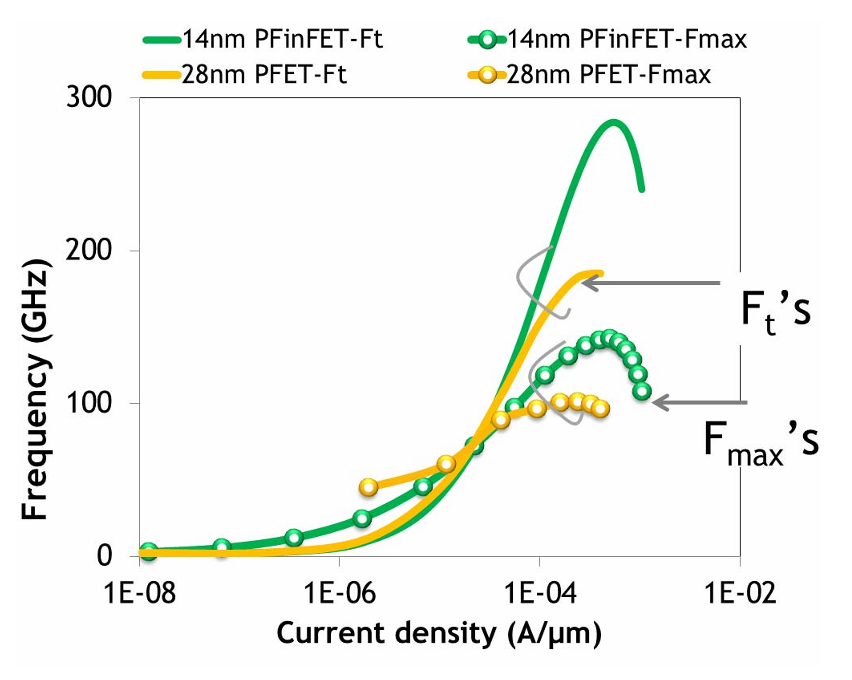
\includegraphics[width=\textwidth]{src/frequencies-ptype.png}
            \end{subfigure}
            \caption{\label{fig:performance-frequencies}Cutoff and maximum oscillation frequencies over current density dependence}
        \end{figure}

        Furthermore, the 14 nm FinFET processing involves the creation of deep silicon cavities for subsequent growing of a boron-doped SiGe epitaxy stressor inside them. The compressive stress over the fin channel boosts the overall hole carrier mobility, hence significantly increasing in the transconductance $G_{\mathrm{m}}$. This directly translates to much higher cutoff frequency and self-gain. The self-gain is further improved during the on-state operation, where a FinFET device experiences full channel depletion. This is thanks to better electrostatic gate control by suppressing the short-channel effects, i.e., the punchthrough and the drain-induced barrier lowering, resulting in lower output conductance $G_{\mathrm{ds}}$.
        
        All the results discussed above are summarized in Table~\ref{table:rf-parameters-comparison} which serves as a good and standing-out comparison of key performance factors.%
            \footnote{The data were taken for a 14 nm RF FinFET and a 28 nm planar FET with a high-K metal gate. The $G_{\mathrm{msat}}$ was measured at $V_{\mathrm{dd}} = \qty{8}{\volt}$. The $S_{\mathrm{vg}}$ is measured at $f = \qty{1}{\kHz}$.}
        \begin{table}[!ht]
            \centering
            \begin{tabular}{|c|c|c|c|c|}
                \hline
                Device & NFinFET & PFinFET & NFET & PFET\\
                \hline\hline
                $f_{\mathrm{t}}$ [$\unit{GHz}$] & 314 & 285 & 308 & 185\\
                \hline
                $f_{\mathrm{max}}$ [$\unit{GHz}$] & 180 & 140 & 159 & 102\\
                \hline
                $G_{\mathrm{msat}}$ [$\unit{\siemens\per\meter}$] & 3017 & 2748 & 985 & 395\\
                \hline
            \end{tabular}
            \caption{\label{table:rf-parameters-comparison}Comparison of key RF parameters between 14 nm FinFET and 28 nm planar FET}
        \end{table}

        For more details on the performance differences between N-type and P-type FinFET devices, related work~\cite{zhang-niu-cai-imura:pmos-nmos-14nm-finfet-comparison} serves as a good elaborate analysis of this topic.

    
    \section{Conclusion}

        The enhancement of FinFET technology's RF and analogue capabilities opens avenues to achieve RF + Logic system-on-chip (SoC) architectures, capitalizing on the technology's strides in logic power, performance, and area scaling.
        
        Moreover, the trend towards digitally assisted analogue designs further highlights the appeal of the FinFET technology, given its scaled footprint and robust digital design portfolio. Consequently, optimized RF SoC designs based on the FinFET technology emerge as an appealing choice~\cite{farley:programmable-rf-soc-in-16nm-finfet-technology-for-broadband-communications}.


    \begin{thebibliography}{20}

        \bibitem{singh:14nm-finfet-analog-and-rf-applications} J. Singh \emph{et al.}, "14-nm FinFET Technology for Analog and RF Applications," in \emph{IEEE Transactions on Electron Devices}, vol. 65, no. 1, pp. 31-37, Jan. 2018, doi: 10.1109/TED.2017.2776838.

        \bibitem{farley:programmable-rf-soc-in-16nm-finfet-technology-for-broadband-communications} B. Farley \emph{et al.}, "A programmable RFSoC in 16nm FinFET technology for wideband communications," \emph{2017 IEEE Asian Solid-State Circuits Conference (A-SSCC)}, Seoul, Korea (South), 2017, pp. 1-4, doi: 10.1109/ASSCC.2017.8240201.

        \bibitem{zhang-niu-cai-imura:pmos-nmos-14nm-finfet-comparison} J. Zhang, G. Niu, W. Cai and K. Imura, "Comparison of PMOS and NMOS in a 14-nm RF FinFET technology: RF Characteristics and Compact Modeling," \emph{2020 IEEE 20th Topical Meeting on Silicon Monolithic Integrated Circuits in RF Systems (SiRF)}, San Antonio, TX, USA, 2020, pp. 47-49, doi: 10.1109/SIRF46766.2020.9040187.
		
	\end{thebibliography}

\end{document}